\documentclass[a4paper, 12pt]{scrreprt}

\pagenumbering{roman}
\setcounter{secnumdepth}{3}
\setcounter{tocdepth}{2} 

\usepackage[german]{babel}
\usepackage[utf8]{inputenc}
\usepackage[T1]{fontenc}
%\usepackage{fancyhdr}
\usepackage{geometry}
\usepackage{lmodern}
\usepackage{verbatim}
\usepackage{graphicx}
\usepackage[pdfborder={0 0 0}]{hyperref}
\usepackage{listings}


\usepackage{caption}

\usepackage{amsmath}
\usepackage{blindtext}


\usepackage{fancybox}
\usepackage{makeidx}% \makeindex
\usepackage{lastpage}
\usepackage{natbib}

%\linespread{1.5}
%\geometry{footskip=40pt}
\setcounter{page}{2}
\linespread{1.25}


\begin{document}

\begin{titlepage}
%\includegraphics[scale=0.3]{Z1.png} \hfill
%\includegraphics[scale=0.1]{2.png}\\[1.8cm]
    \begin{center}
    \LARGE \textbf{VirtualDesktop} \\
    \vspace{2.5cm}
    \large\textbf{Projekt}\\
    \vspace{2.5cm}
    \normalsize
    Hochschule RheinMain Wiesbaden \\
    \vspace{2cm}
    \large \textbf{Fortgeschrittene Themengebiete der Informatik\\ Cloud Computing\\}
    \vspace{1cm}
    \normalsize
    Abgabedatum: 30. Januar 2019\\
    \vspace{2.7cm}
    \end{center}
 \normalsize{
    \begin{tabular}{ll}
    	Gruppe: & \\
    	Robin Bergfeld & \\
    	Abiram Pakeerathan & \\
    	Simon Rininsland & \\[0.5cm]
    	Dozent: &\\
        Prof. Dr. Philipp Schaible & \\
    \end{tabular}
    }
\end{titlepage}



\clearpage
\tableofcontents
\clearpage

\pagenumbering{arabic}

%zitieren:
% \cite{Joa10:1}

\chapter{Einführung}
%Mit was, wer wo...
Im Rahmen dieses Projektes ist eine Web-Anwendung unter Verwendung von Amazon Web-Services (AWS) entwickelt worden. Zunächst wird in diesem Kapitel die Idee vorgestellt, anschließend wird die Architektur und die Umsetzung thematisiert.

\section{Projektanforderungen}
%- Welche Anforderungen vom Modul\\
%- Fokus des Projekts




\section{VirtualDesktop}
%- Was mit Bildern (kurz, vielleicht nur ein Bild)\\
%- Funktionen erläutern (MultiWindow, Benutzerverwaltung inkl Rechteverwaltung, Stream, Up-Download, Show)\\
%- Ziel des Produkts (müssen sich mit Anforderungen des Moduls decken)\\

Die Web-Anwendung \textit{VirtualDesktop} soll registrierten Benutzern virtuelle Desktops zur Verfügung stellen, die auf jedem Gerät aufrufbar sind und mit anderen Benutzern geteilt werden können. Die erstellten Desktops sollen zur Multimediaablage genutzt werden. Der Up- und Download ist mit beliebigen Dateitypen möglich. Zusätzlich können Bilder angezeigt sowie Audio- und Video-Daten gestreamt werden.\\[0.25cm]
Alle Benutzer müssen sich anmelden um die Anwendung nutzen zu können. Ein Benutzer kann mehrere Desktops anlegen und diese verwalten. Das Anlegen von mehreren Desktops ist zum Beispiel dann sinnvoll, wenn die Desktops mit unterschiedlichen Personengruppen geteilt werden sollen.
Für jeden angelegten Desktop, kann der Ersteller andere Nutzer hinzufügen und ihnen verschiedene Rechte an seinem Desktop zuweisen.\\
Mit zugewiesenen Leserechten kann der Nutzer Dateien betrachten und herunterladen, mit Schreibrechten darf der Nutzer auch eigene Dateien auf diesem Desktop ablegen. Dem Nutzer müssen explizit Löschrechte zugewiesen werden, um Dateien von fremden Desktops entfernen zu können.\\
Nutzer können auch Admin-Rechte erhalten, sodass diese für den Desktop Nutzerrechte bearbeiten und neue Nutzer hinzufügen dürfen. Ein angelegter Desktop kann aber ausschließlich nur vom Ersteller entfernt werden.\\ 
Es gibt also
\begin{itemize} 
\item[] \textbf{Owner}, die einen oder mehrere Desktops angelegt haben, zwischen diesen wechseln können und andere Nutzer durch Zuweisung von Lese- , Schreib- und Löschrechten zu ihren Desktops hinzufügen dürfen. Sie besitzen für ihre eigenen Desktops alle Rechte. Sie können auch Admin-Rechte, für die Bearbeitung von Nutzerrechten, vergeben.
\item[] \textbf{User}, die Rechte für einen oder mehrere Desktops zugewiesen bekommen haben und zwischen diesen wechseln können und diesen Rechten entsprechend Aktionen ausführen dürfen.
\end{itemize} 


\begin{figure}[h]
\centering
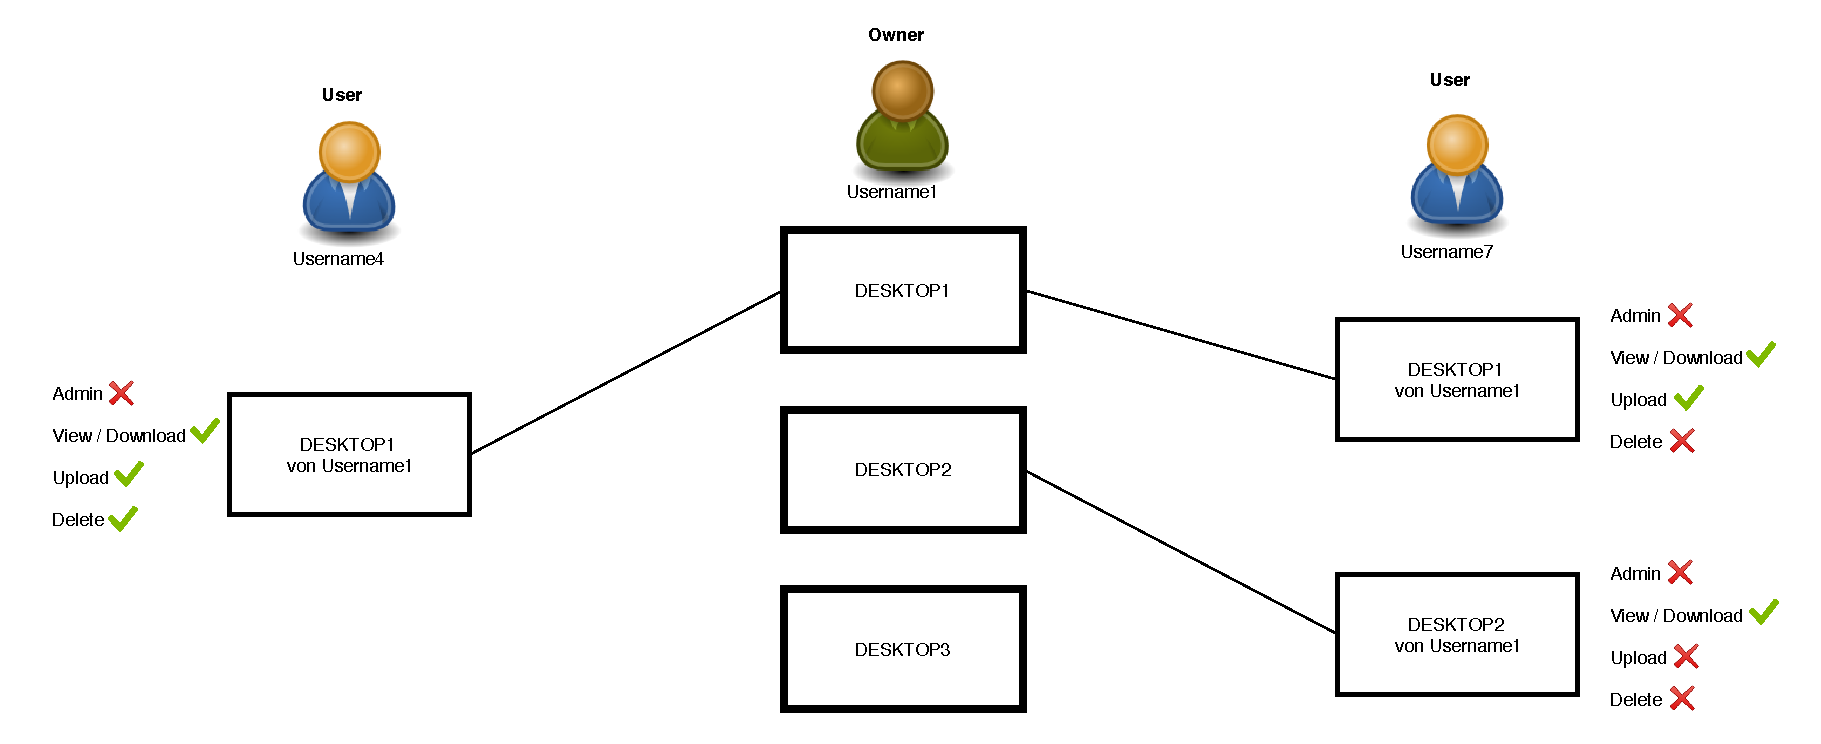
\includegraphics[scale=0.45]{VD_konzept.pdf}
\caption{Username1 ist Owner und besitzt drei Desktops. DESKTOP1 teilt Username1 mit Username4 und Username7. Der DESKTOP2 wird nur mit Username7 geteilt. Den Usern wurden individuell für diese Desktops Rechte zugeteilt. Den DESKTOP3 kann nur der Owner selbst betrachten.}
\end{figure}

\chapter{Weg in die Cloud}
MIT Sections
-was man alles brauch um einen webservice zu bauen: SERVER mit db und Webserver (Aufbau klassischer Webservice)
- Skalierbarkeitswunsch: aufsplittung des SERVERS in Speicher, Rechenleistung, DB, Authentifizierung, ... UND DESHLAB GIBT ES ZB. NOSQL DATENBANKEN
- outsourcing zu einem cloudservice/beschreibung kontrollverlust IaaS-PaaS-SaaS-FaaS (wieso man es in andere hände gibt/Kosten/..)
- aufllistung von einigen cloudanbieter AWS, Azure, Google...


\chapter{Architektur}
%- Festlegung auf AWS
%- architeturdiagramm
%- Struktur DB und Struktur Anwendungskommunikation- Zusammenhang

Im folgendem wird die Architektur der Webanwendung VirtualDesktop unter Verwendung von Amazon Web Services als Architekturdiagramm dargestellt.

\textbf{[BILD EINFÜGEN TODO]}


\section{Elastic Beanstalk Konfiguration}
%-config file
%-  Inkl aller Subservices die EBS anlegt.(LoadBalancer, Security Groups, S3 Bucket für EB Code, Cloudwatch)
%- was es alles mit drin hat aber nebenbei erwähnen immer wieso und
- [WOFÜR IST DIE DATEI GUT? EINLEITEND ERKLÄREN]



\subsection{Authentifizierungsservice Cognito}
Zur Authentifizierung von Nutzern wird der AWS Cognito verwendet. Der Nutzerpool \textit{Cognitopool} vom Typ \textit{AWS::Cognito::UserPool} ist so konfiguriert, dass bei der Registrierung eines neuen Nutzers ein Passwort angegeben werden muss, welches die Minimalvorrausetzung eines AWS-Cognito-Passworts erfüllt (Zeichenlänge von Sechs[QUELLE: AWS COGNITO]). Für die Registriereung muss der Nutzer sich verifizieren. Dies geschieht hier über Email,in der der Nutzer seinen Bestätigungscode erhält. Die Formatierung dieser Email wird in \textit{EmailVerificationMessage} und \textit{EmailVerificationSubject} angegeben.  
%COGNITO MINLÄNGE
%https://docs.aws.amazon.com/de_de/AWSCloudFormation/latest/UserGuide/aws-properties-cognito-userpool-passwordpolicy.html

 

\begin{lstlisting}[xleftmargin=\parindent,numbers=left,numberstyle=\small,numbersep=8pt,frame=L,mathescape=true, basicstyle=\small, language=Java, lineskip={1.0pt}]
CognitoPool:
        Type: AWS::Cognito::UserPool
        Properties:
            AutoVerifiedAttributes:
                -
                    "email"
            EmailVerificationMessage: "Here is your code: {####}"
            EmailVerificationSubject: "Verify your E-Mail for VD"
            Policies:
                PasswordPolicy:
                    MinimumLength: "6"
                    RequireLowercase: false
                    RequireNumbers: false
                    RequireSymbols: false
                    RequireUppercase: false

\end{lstlisting}
\bigskip
\noindent Um den \textit{UserPool} verwenden zu können, benötigt dieser einen Benutzer, den \textit{AWS::Cognito::UserPoolClient}. Dieser wird über die Property \textit{UserPoolId} an den angegeben \textit{UserPool} gebunden, in diesem Fall wird eine Referenz auf den zuvor angelegten UserPool mit dem Namen \textit{CognitoPool} angegeben. Die Property \textit{GenerateSecret} wird hier auf \textit{false} gesetzt, da die clientseitig verwendete Amazon Cognito Identity-SDK für JavaScript keine client secrets unterstützt [QUELLE: generateSec].
%generateSec QUelle
%https://github.com/aws-amplify/amplify-js/tree/master/packages/amazon-cognito-identity-js

\begin{lstlisting}[xleftmargin=\parindent,numbers=left,numberstyle=\small,numbersep=8pt,frame=L,mathescape=true, basicstyle=\small, language=Java, lineskip={1.0pt}]
    CognitoClient:
        Type: AWS::Cognito::UserPoolClient
        Properties:
            GenerateSecret: false
            UserPoolId: '{"Ref" : "CognitoPool"}'
\end{lstlisting} 


\subsection{Could-Speicher S3}
Durch folgende Beschreibung in der Konfiguration wird ein Cloud-Speicher des Typs \textit{AWS::S3::Bucket} angelegt.
\begin{lstlisting}[xleftmargin=\parindent,numbers=left,numberstyle=\small,numbersep=8pt,frame=L,mathescape=true, basicstyle=\small, language=Java, lineskip={1.0pt}]
Bucket:
        Type: AWS::S3::Bucket
\end{lstlisting}          


\subsection{Datenbank DynamoDB}
Zur Erstellung einer Datenbanktabelle in der DynamoDB wird hier exemplarisch an der \textit{Permissions}-Tabelle vom Typ \textit{AWS::DynamoDB::Table} gezeigt. Anders als bei klassischen SQL-Datenbanken kann ein Eintrag in einer DynamoDB-Tabelle beliebige Felder beinhalten. Diese werden lediglich über den Schlüssel abgefragt. Um den Schlüssel einer Tabelle zu definieren muss der Attributtyp, der Attributname und der Keytyp innerhalb der AttributeDefinitions und KeySchema angegeben werden. Diese beiden Felder sind erforderlich, müssen also angegeben werden. Das selbe gilt für \textit{ProvisionedThroughput}[QUELLE allg.DYNDB ].
Dies bedeutet, dass die Skalierung kann nicht bei der Erstellung durch CloudFormation oder EBS eingestellt werden. Um die DynamoDB zu skalieren muss \textit{AWSServiceRoleForApplicationAutoScaling\_DynamoDBTable} im AWS-Account aktiv sein. Falls \textit{AWSServiceRoleForApplicationAutoScaling\_DynamoDBTable} bereits bei der Erstellung durch EB-Deploy aktiviert war skalieren die Tabellen ansonsten nicht. Das Autoscaling für die Tabellen kann dann jedoch nachträglich über die Management-Console eingestellt werden. Nähere Informationen hierzu sind in [QUELLE: AUTOSCALING] zu finden.

%QUELLE allg.DYNDB
%https://docs.aws.amazon.com/de_de/AWSCloudFormation/latest/UserGuide/aws-resource-dynamodb-table.html


%QUELLE AUTOSCALING
%https://docs.aws.amazon.com/de_de/amazondynamodb/latest/developerguide/AutoScaling.Console.html


\begin{lstlisting}[xleftmargin=\parindent,numbers=left,numberstyle=\small,numbersep=8pt,frame=L,mathescape=true, basicstyle=\small, language=Java, lineskip={1.0pt}]
Permissions:
        Type: AWS::DynamoDB::Table
        Properties:
            AttributeDefinitions:
                -
                    AttributeName: "Window"
                    AttributeType: "S"
                -
                    AttributeName: "User"
                    AttributeType: "S"
            KeySchema:
                -
                    AttributeName: "Window"
                    KeyType: "HASH"
                -
                    AttributeName: "User"
                    KeyType: "RANGE"
            ProvisionedThroughput:
                ReadCapacityUnits: "1"
                WriteCapacityUnits: "1"
\end{lstlisting}



\subsection{Serverless-Functions Lambda}

\section{Zusammenhang der Services}
%- über NodeJS und Express(wegen Datentransformation JSON) ...
%- Auth und Berechtigung prüfen- setzen von Rechten
%- wie sehen die Tabellen aus
%- wie findet das Computing statt
%- kurz jede api-Funktion anreißen
%













\chapter{Besonderheiten}
Einleitung dazu: Weil zu viel gemacht - nur die interessante Teile näher erklärt.

\section{Entwicklungsumgebung lokal / Env- Variablen in NodeJS}
%- Was ist das Problem.\\ 
%- Wie haben wir es gelöst\\
%-  z.B. www Cognito

Bei Elastic-Beanstalk-Projekten wird bei jedem Deploy die gesamte Umgebung mit allen AWS-Resourcen neu gestartet. Dies beinhaltet unter anderem die EC2-Instanz. Da bei Quellcodeänderungen ein Deploy erneut ausgeführt werden muss und die Instanziierung einer EC2-Instanz zeitaufwendig sein kann ist dies für die Entwicklung der Webanwendung nicht praktikabel. Aus diesem Grund wurden in Elastic-Beanstalk Referenzen[QUELLE: REF AWS] für die dynamisch angelegten Ressourcen erzeugt. Diese Referenzen können in Umgebungsvariablen der EC2-Instanzen übernommen werden, dies geschieht in der \textit{node-env-keys.config} [QUELLE: ENVI VAR].\\
Um eine schnellere Entwicklung voranzutreiben wird dieser Umstand genutzt, indem statische (nicht durch EBS-Deploy generiert) Amazon Web Services erstellt und in die Umgebungsvariablen des Entwicklersystems hinzugefügt werden.
Hierbei ist zu beachten, dass lediglich die EC2-Instanzen durch den lokalen Rechner ersetzt werden. Anzulegende Umgebungsvariablen sind
AWS\_ACCESS\_KEY\_ID und AWS\_SECRET\_ACCESS\_KEY mit den AWS-Credials, COGNITO\_CLIENT und COGNITO\_POOL mit der App-Client-ID eines Cognito-Clients (mit GenerateSecret=false) und der Pool-ID des dazugehörigen Cognito-Pools, FILES, PERMISSIONS und WINDOWS mit den jeweiligen Tabellennamen von DynamoDB-Tabellen mit der Struktur beschrieben in [.\textbf{TODO}.] und BUCKET sowie THUMB\_BUCKET mit den Bucket-Namen. Weiterhin muss die Lambda-Funktion wie in \textbf{LAMDBA TODO} beschrieben  für die Generierung von Thumbnails erstellt werden. Die Lambda-Funktion muss mit den Buckets verknüpft sein.  


%REF QUELLE
%https://docs.aws.amazon.com/de_de/AWSCloudFormation/latest/UserGuide/intrinsic-function-reference-ref.html

%EVI VAR
%https://docs.aws.amazon.com/de_de/elasticbeanstalk/latest/dg/environments-cfg-softwaresettings.html



\section{DynamoDB}
%- Was ist das Problem. Nicht mehrere Sachen löschen nicht möglich.
Da die DynamoDB nicht über die Möglichkeit verfügt, mehrere Einträge über einen Key zu entfernen, muss für die \textit{deleteWindow}-Funktion die gesamte \textit{File}-Liste und \textit{Permission}-Liste für den gegebenen Key eingelesen und jeder Eintrag einzeln in der DynamoDB entfernt werden.
Um nicht jeden Listeneintrag einzeln zu entfernen kann zwar \textit{batchWriteItem} verwendet werden, dieses ist jedoch max. auf 25 DeleteItem-Operationen limitiert und es können keine \textit{conditions} angegeben werden [QUELLE: DELTEEITEM]. Aus diesem Grund werden die Items, wie hier einleitend erwähnt, einzeln entfernt.

%deleteITEM AWS
%https://docs.aws.amazon.com/AWSJavaScriptSDK/latest/AWS/DynamoDB.html#deleteItem-property

\section{Promise / Dispatcher}
%- Was ist das Problem. Wofür brauchen wir das. Wo war das problem.\\
%- Erklären wieso wieso wir das bauen.\\
%- Erklären was wir gebaut haben und wie.\\
%- kann easy erweitert werden


Die Funktion der AWS-sdk arbeiten mit Callbacks, jedoch sind Aufgaben wie z.B. das Löschen von Desktops und deren Inhalt parallelisierbar, und müssen synchronisiert werden. Um dies zu bewerkstelligen, und um komplexe Callbackstrukturen zu vermeiden wurde eine \textit{dispatch}-Funktion für solche Aufgaben konzipiert. 

\begin{lstlisting}[xleftmargin=\parindent,numbers=left,numberstyle=\small,numbersep=8pt,frame=L,mathescape=true, basicstyle=\small, language=Java, lineskip={1.0pt}]
async function dispatch(tasks, map, callback) {
    var data = { tasks: tasks,
                 map: map, 
                 result: {}, 
                 errors: [], 
                 propergate: true 
    };
    while(data.tasks.length != 0 && data.propergate) {
        var promises = [];
        for (var i = 0; i < tasks[0].length; i++) {
            var f = function(resolve, reject) {
                    this.tasks[0][i](this, () => {
                    resolve();
                });
            };
            promises.push(new Promise(f.bind(data)))
        }
        await Promise.all(promises);
        data.tasks.splice(0, 1);
    }
    callback(data);
}
\end{lstlisting}

Es wird hier zum einen der Parameter \textit{tasks}, einem Array aus Arrays aus Funktionen, der Form \textit{(dis, done)}, sowie ein Objekt \textit{map}, welches innerhalb der \textit{tasks} über \textit{dis.map} zugreifbar ist, und einer \textit{callback}-Funktion, welche nach Beendigung aller \textit{tasks} ausgeführt und die Resultate und Fehler zurückliefert, übergeben. Der \textit{callback} ist notwendig, da die Funktion asynchron ist. Die \textit{dispatch}-Funktion sorgt dafür, dass die Funktionen der inneren \textit{task}-Arrays parallel durch die Kapslung in \textit{promisses} ausgeführt werden. Der Array selbst wird sequentiell ausgeführt, dies wird durch \textit{await} sichergestellt. Es ist zu dem möglich, während des \textit{dispatch}-Prozesses weitere \textit{tasks} hinzuzufügen (dies wird z.B. beim Löschen von Desktops verwendet). Ermöglicht wird dies, da jede \textit{(dis, done)}-Funktion auf das \textit{data}-Objekt und somit auf das Doppelarray aus Funktionen zugreifen kann. Dadurch ist es den Funktionen auch möglich, Ergebnisse in \textit{results} zu speichern, Fehler in \textit{errors} anzugeben und die weitere Ausführung paralleler Arbeitsschritte durch das setzen von \textit{propergate} auf false zu verhindern. Das \textit{dis} der \textit{(dis, done)}-Funktion wird hierbei auf \textit{data} gebinded, das \textit{done} ist hier eine \textit{callback}-Funktion, welche das \textit{resolve} von \textit{Promise} ausführt. Die Funktion \textit{dispatch} kann wie am folgendem Beispiel der \textit{deleteWindow}-Funktion gezeigt verwendet werden:

\begin{lstlisting}[xleftmargin=\parindent,numbers=left,numberstyle=\small,numbersep=8pt,frame=L,mathescape=true, basicstyle=\small, language=Java]

function deleteWindow(username, windowName, callback) {
    var map = { 
        "username": username, 
        "windowName": windowName
    };
    dispatch([[checkParams], 
              [getPermissions], 
              [checkPermissions("owner")], 
              [deleteWindowDynamoDB, 
               removeFilesAndFileInfos, 
               deleteWindowPermissonsDynamoDB
             ]], map, (data) => {
        callback(reply(data));
    });
}
\end{lstlisting}

\noindent Zunächst wird der \textit{username} und \textit{windowName} durch \textit{checkParams} auf Existenz geprüft. Anschließend werden die Berechtigungen für den Benutzer durch \textit{getPermissions} aus der DynamoDB für den angegeben Desktop abgefragt. Die Berechtigungen sind nun im Kontext von \textit{checkPermissions} über \textit{dis.data} zugreifbar. Die \textit{checkPermissions}-Funktion setzt \textit{propagate} auf \textit{false}, falls der Nutzer nicht Besitzer des Desktops ist (und einen Fehler in \textit{dis.errors}-Array schreiben). Ansonsten wird der Desktop und alle dazugehörigen Inhalte und Berechtigungen gelöscht.    

\section{Model-View-Controller}
%- Warum brauchen wir das\\
%- kann easy erweitertert werden\\
%- Wie haben wir es gelöst

Um parallele Entwicklung des Projektes gewährleisten zu können wird ein Model-View-Controller verwendet. Das Model beinhaltet hierbei die Amazon Web Services S3, DynamoDB, Cognito welche durch die \textit{virtual-desktop.js} in Schnittstellen abstrahiert wird und mittels NodeJS-Express-Server für den Controller zugänglich ist. Diese Abstraktion wurde vorgenommen, damit der NodeJS-Express-Server durch AWS-Lambda substituiert werden kann. Der NodeJS-Express-Server wird durch den Elastic-Beanstalk bereitgestellt. AWS-Lambda wird im Backend verwendet um für neue Dateien, welche durch den Nutzer in den S3-Bucket gespeichert werden Thumbnails zu erstellen.\\
Die Schnittstelle \textit{api.js} im Frontend wird durch den Controller erweitert. Dieser Controller reagiert auf die Eingaben des Nutzers im Frontend, indem Controller-Funktionen angesprochen werden. Bei Bedarf werden Backend-Funktionen durch den Controller angesprochen und/oder im Frontend Events ausgelöst, wodurch dieses aktualisiert werden kann.
Die Verwendung eines Controllers ist vorteilhaft um die spätere Einbindung von Push-Notifications mit geringem Aufwand zu realisieren.



\section{Streaming Download / Upload}
%- Was ist das Problem. Wofür brauchen wir das. Wo war das problem.\\
%- Erklären wieso wieso wir das bauen.\\
%- Erklären was wir gebaut haben und wie.

Um Dateien von und in den S3-Bucket zu laden, können Buffer verwendet werden, dies bedeutet das die Dateien zunächst im Arbeitsspeicher oder im Speicher des NodeJS-Express-Server zwischengespeichert werden müssen. Da eine EC2-Instanz nur über ein begrenztes Volumen an Speicher verfügt, ist das Buffern von Dateien nicht empfehlenswert (erhöhte Kosten, Skalierung von EC2-Instanzen) [QUELLE: EC2 AWS].\\
%https://aws.amazon.com/de/ec2/pricing/on-demand/
Aus diesem Grund werden die Dateien in diesem Projekt vom Backend gestreamt. Hierzu wurden die folgenden Express-Middleware-Bibliotheken geprüft:

\begin{itemize}
\item multer
\item express-fileupload
\item express-busboy
\item busboy-body-parser
\item busboy
\end{itemize}


%TO DO: QUELLEN EINTRAGEN - in .BIB
\noindent Die Middleware \textit{multer} und \textit{express-fileupload} kommen für das gestreamte Hochladen von Dateien auf den S3-Bucket nicht in Frage, da sie keine Streams unterstützen sondern entweder auf der Festplatte speichern  oder im Arbeitsspeicher buffern [quelle: multer, fileupload].
%multer: https://www.npmjs.com/package/multer
%fileupload: https://www.npmjs.com/package/express-fileupload
Um \textit{busboy} im Kontext von NodeJS-Express verwenden zu können, kann \textit{express-busboy} verwendet werden. Allerdings ist diese Bibliothek ebenfalls nur im Stande auf die Festplatte zu speichern. Auch der \textit{busboy-body-parser} stellte sich bei näherer Betrachtung des Quellcode als ungeeignet heraus, da auch dieser nur im Arbeitsspeicher buffert [QUELLE: busboy-body-parser].\\
Die Bibliothek \textit{busboy} hingegen liest den HTTP-Request als Stream ein und bietet auch die Dateien als Stream an [QUELLE BUSBOY].
%https://www.npmjs.com/package/busboy
Die Problematik, die sich hieraus ergibt, ist das für das Speichern der Datei der Desktop auf dem die Datei gespeichert werden soll bekannt sein muss. Da \textit{busboy} allerdings auf dem HTTP-Request-Stream arbeitet muss der Desktopname vor der Datei im \textit{multipart/form-data} stehen. Um \textit{busboy} zu verwenden wurde daher eine minimalistische Middleware \textit{busboySync.js} entwickelt [QUELLE MIDDLEWARE].
%https://expressjs.com/en/guide/using-middleware.html
Diese Middleware kommt in allen Resourcen als Router-Middleware des NodeJS-Express-Servers zum Einsatz, welche \textit{multipart/form-data} verarbeitet. Ausnahme hierbei bildet die \textit{/addFile}-Resource, welche aus oben genannten Gründen \textit{busboy} nativ verwendet.\\
Für den Download von Dateien wird die \textit{/getStream}-Resource verwendet, diese liefert für typische Range-Requests der Form
\begin{lstlisting}
bytes=x-y
\end{lstlisting}
, wobei x das Start-byte und y das End-byte darstellt (y kann auch entfallen), ein HTTP-Response-206 (Partial Content) zurück [QUELLE: Range,206 7233].
%https://www.rfc-editor.org/rfc/rfc7233.txt 



%busboy-body-parser
%https://github.com/lennym/busboy-body-parser/blob/master/index.js

\section{Lambda - Thumbnailgenerator}
- Was macht das\\
- Wie geht das

\chapter{Kosten - Aufwände}

\section{Laufkosten}
- Aufführung der genutzten Services mit Bezug auf Kosten\\
- Hochrechnung pro Monat und pro Nutzer (oder pro 100 Nutzer) \\
- Grafik erstellen







\clearpage
\bibliography{documentation}
%\bibliographystyle{apalike}

\end{document}